\chapter{Własne propozycje algorytmów}

\noindent Od początku istnienia tematyki eksploracji strumieni danych powstało w tej dziedzinie wiele algorytmów próbujących stale podnosić poziom trafności klasyfikacji. Coraz to nowsze implementacje starają się wykorzystywać najnowsze elementy z dziedziny uczenia maszynowego jak np. sieci neuronowe. Mimo tego faktu w dziedzinie przetwarzania strumieni danych nadal istnieją takie typy strumieni danych, z których klasyfikacją nie radzą sobie najlepiej algorytmy dostępne na rynku. Ta obserwacja z kolei powoduje zwiększenie zainteresowania wśród badaczy poprzez podejmowanie kolejnych prób rozszerzenia czy też stworzenia nowych algorytmów, które poradziłyby sobie z klasyfikacją problematycznych strumieni danych.

Wspomniana obserwacja była także motywacją do zgłębienia tematyki strumieni danych, próby stworzenia nowych podejść do klasyfikacji danych oraz powstania niniejszej pracy. W ramach tego rozdziału przedstawione zostaną trzy nowe algorytmy skupiające się na klasyfikacji niezbalansowanych i zmiennych strumieni danych: \textit{Neighbourhood Oversampling Online Bagging (NOOB)}, \textit{Neighbourhood Undersampling Online Bagging (NUOB)} oraz \textit{Hybrid Neighbourhood Online Bagging (HNOB)}. Odpowiednio pierwsze z podejść jest rozszerzeniem wcześniej przedstawionego algorytmu \textit{Oversampling Online Bagging (OOB)}, drugie podejście rozszerza algorytm \textit{Undersampling Online Bagging (UOB)}, a trzecie z podejść jest hybrydą łączą podejścia zaprezentowane w algorytmach \textit{NOOB} oraz \textit{NUOB}.

Wszystkie zaprezentowane w tym rozdziale algorytmy zostały zaimplementowane w języku \textit{Java} przy pomocy wcześniej już wspomnianej biblioteki \textit{Massive Online Analysis (MOA)} \cite{Article:MOA}. Wszystkie szczegóły dotyczące implementacji oraz kodu źródłowego zostały zawarte w repozytorium, dostępnym jako załącznik \ref{Chapter:Repository} do rozprawy.

\newpage

\section{Neighbourhood Oversampling Online Bagging}

\noindent Pierwszym z proponowanych algorytmów jest algorytm \textit{Neigbourhood Oversampling Online Bagging (NOOB)}. Tak jak wcześniej wspomniano algorytm ten jest rozszerzeniem algorytmu \textit{Oversampling Online Bagging} i wykorzystuje technikę \textit{oversampling'u} do zbalansowania liczności przykładów między poszczególnymi klasami. Aby lepiej przeanalizować modyfikacje, które wprowadza proponowane podejście, w sekcji \ref{Algorithm:NOOB} przedstawiono pseudokod algorytmu.

\begin{algorithm}
    \caption{Neighbourhood Oversampling Online Bagging}\label{Algorithm:NOOB}
    \textbf{Input}: $S$: stream of examples \\
    \hspace*{12mm} $n$: number of classifiers in ensemble \\
    \hspace*{12mm} $W$: window of examples \\
    \hspace*{12mm} $k$: number of nearest neighbours \\
    \hspace*{12mm} $\Psi$: additional coefficient for calculating safe level \\
    \textbf{Output}: $\mathcal{E}$: an ensemble of classifiers \\
    \begin{algorithmic}[1]
    \State initialize window $W$
    \State $\mathcal{E} \gets n$ incremental classifiers
    \ForAll{examples $x^t \in S$ \do}
    \State update currenct class size $w^{(t)} = (w^{(t)}_{+}, w^{(t)}_{-})$
    \State calculate safe level of incoming example $L^2_{min} = \frac{(N_{maj}')^\Psi}{k}$
    \If{$y_t$ = $+1$ and $w^{(t)}_{+} < w^{(t)}_{-}$}
    \vspace{0.5em}
    \State $\lambda \gets (w^{(t)}_{-}/w^{(t)}_{+}) \cdot (L^2_{min} + 1)$
    \vspace{0.5em}
    \ElsIf{$y_t$ = $-1$ and $w^{(t)}_{-} < w^{(t)}_{+}$}
    \vspace{0.5em}
    \State $\lambda \gets (w^{(t)}_{+}/w^{(t)}_{-}) \cdot (L^2_{min} + 1)$
    \vspace{0.4em}
    \Else
    \State $\lambda \gets 1$
    \EndIf
    \ForAll{classifiers $C_i \in \mathcal{E}$ \do}
    \State set $l$ $\sim Poisson(\lambda)$
    \For{1 to $l$ \do}
    \State update $C_i$ using $x^t$
    \EndFor
    \EndFor
    \State $W \gets W \cup \{x^t\}$
    \State if necessary remove outdated examples from $W$
    \EndFor
    \end{algorithmic}
\end{algorithm}

\noindent Pierwszą różnicą, którą można zauważyć pomiędzy algorytmem \textit{NOOB} a algorytmem \textit{OOB} jest dodanie kilku dodatkowych zmiennych. Do zmiennych tych należą:

\begin{itemize}
    \item $W$ - okno przesuwne zawierające ostatnie przykłady, które pojawiły się w strumieniu
    \item $k$ - liczba najbliższych sąsiadów wykorzystywanych do obliczania poziomu bezpieczeństwa (\english{safe level}) aktualnie przetwarzanego przykładu
    \item $\Psi$ - dodatkowy parametr wykorzystywanu przy obliczaniu poziomu bezpieczeństwa (\english{safe level}) aktualnie przetwarzanego przykładu
\end{itemize}

\noindent Pierwszym z nowych aspektów, który pojawił się w algorytmie, jest aspekt wprowadzenia okna przesuwnego. Okno przesuwne w tym przypadku odpowiedzialne jest za przechowywanie określonej liczby przykładów, które jako ostatnie pojawiły się w strumieniu. Okno to, w prezentowanym podejściu, wykorzystywane jest do obliczeń liczności przykładów w określonym momencie w czasie (\textit{current class size}) oraz do obliczania poziomu bezpieczeństwa danego przykładu (\textit{safe level}).

Należy zwrócić uwagę na fakt, że we wcześniej prezentowanym algorytmie \textit{OOB} liczności przykładów danych klas były obliczane za pomocą specjalnego wzoru na całym strumieniu danych z wykorzystaniem współczynnika zapominania działającego na najstarsze przykłady w strumieniu - zastosowanie efektu wygładzania wykładniczego. W prezentowanym podejściu algorytmu \textit{NOOB} liczności przykładów danych klas obliczane są na wcześniej przygotowanym oknie zawierającym określoną liczbę ostatnich elementów, które wystąpiły w strumieniu. Motywacją do wprowadzenia takiej modyfikacji była kwestia, że w wielu przetestowanych przypadkach testowych starsze dane, występujące jeszcze przed zjawiskiem dryfu pojęć, zbyt mocno wpływały na późniejsze obliczenia parametru $\lambda$ dla przykładów, które pochodziły z zupełnie innego pojęcia (po wystąpieniu dryfu), mimo zastosowania współczynnika zapominania. Oba wymienione podejścia, co do obliczania liczności przykładów zostały przetestowane dla wygenerowanych strumieni danych i po analizie wyników obu podejść zdecydowano się na podejście z wykorzystaniem obliczeń na podstawie okna przesuwnego. Wyniki obu modyfikacji zostały zawarte w repozytorium dostępnym jako dodatek \ref{Chapter:Repository} do pracy.

Kolejnym aspektem, który został wprowadzony w prezentowanym algorytmie \textit{NOOB}, jest wprowadzenie obliczania poziomu bezpieczeństwa (\english{safe level}) dla aktualnie przetwarzanego przykładu. Dla wcześniej zaprezentowanego algorytmu \textit{OOB} obliczenie parametru lambda korzystało jedynie z wartości liczności przykładów danych klas w określonej chwili czasu $(w^{(t)}_{+}, w^{(t)}_{-})$. Obserwacja ta determinowała fakt, że algorytm skupia się głównie na celu zbalansowania obu klas i nie zwraca uwagi na ich rozkład, wobec czego można założyć hipotezę, że podejście to nie będzie w stanie sobie poradzić z dodatkowymi czynnikami trudności takimi jak np. napływ przykładów określonego typu czy przemieszczanie się skupisk przykładów klasy mniejszościowej. Aby zapobiec temu problemowi w prezentowanym algorytmie \textit{NOOB} zdecydowano się na wprowadzenie aspektu poziomu bezpieczeństwa.

Motywacją do wprowadzenia cechy poziomu bezpieczeństwa był artykuł \cite{Article:NNBag}, w którym autorzy podejmują problem radzenia sobie z niezbalansowanymi danymi w uczeniu maszynowym z danych statycznych. Szczegółowo zwracają uwagę na dodatkowe czynniki, które należy wziąć pod uwagę podczas procesu uczenia, aby poprawić trafność klasyfikacji na istniejących zbiorach danych. Końcowym efektem ich pracy jest propozycja nowego podejścia nazwanego \textit{Neighbourhood Balanced Bagging (NBBag)}, które w głównej mierze manipuluje prawdopodobieństwem wylosowania określonego przykładu do próbki typu \textit{bootstrap}. Jednym ze składowych elementów do obliczenia prawdopodobieństwa jest obliczenie poziomu bezpieczeństwa określonego przykładu (\english{safe level}). Formuła do obliczania poziomu bezpieczeństwa prezentuje się następująco:

\begin{equation}
    L^2_{min} = \frac{(N_{maj}')^\Psi}{k}
\end{equation}

\noindent gdzie:

\begin{itemize}
    \item $k$ - liczba najbliższych sąsiadów wziętych do analizy (parametr algorytmu)
    \item $N_{maj}'$ - liczba przykładów należących do klasy większościowej spośród k najbliższych sąsiadów
\end{itemize}

\noindent Jednym z parametrów przedstawionego powyżej wzoru jest parametr $\Psi$, który odpowiedzialny jest za dodatkową manipulację wartościami poziomu bezpieczeństwa danego przykładu.

\begin{figure}[h]
    \centering
    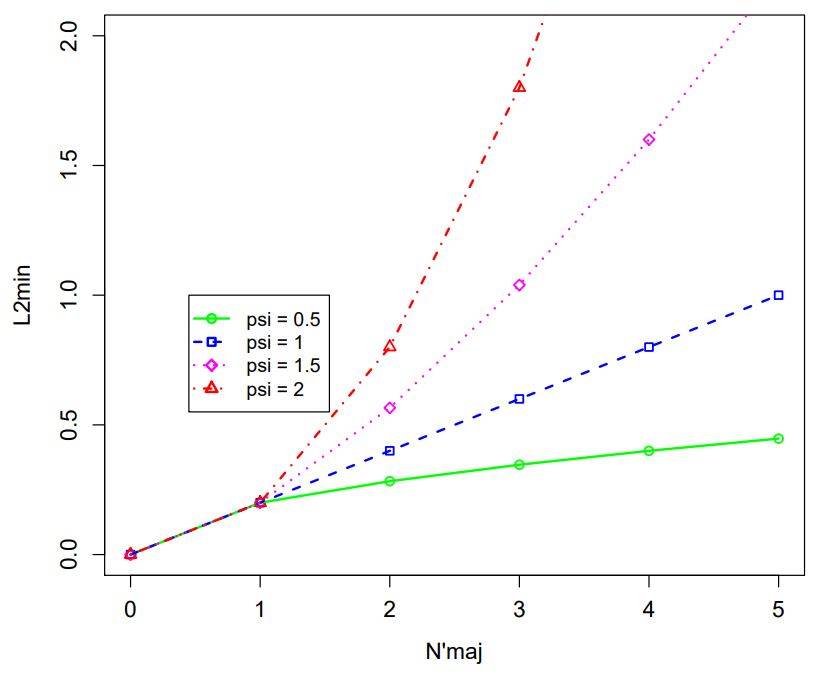
\includegraphics[width=13cm]{figures/psi_coeff.JPG}
    \caption{Wykres pokazujący różnice między wartościami miar $L^2_{min}$ w zależności od parametru $\Psi$ \cite{Article:NNBag}}\label{Figure:PsiCoefficient}
\end{figure}

\noindent Jak można zauważyć na rysunku celem wprowadzenia dodatkowego parametru $\Psi$ jest zwiększenie wartości miary $L^2_{min}$ w zależności od liczby przykładów z klasy większościowej, którymi dany przykład jest otoczony. W ten sposób położony jest jeszcze większy nacisk na poprawną klasyfikację przykładów, które oznaczone są jako rzadkie (\english{rare}) oraz odstające (\english{outlier}). 

Warto też zwrócić uwagę na okoliczność, że wspomniany poziom bezpieczeństwa dla określonego elementu w środowisku strumieniowym obliczany jest na podstawie wcześniej przywołanego okna przesuwnego zawierające określoną liczbę najświeższych przykładów. Ocena liczby $k$ najbardziej podobnych przykładów do aktualnie przetwarzanego przykładu wykonywana jest z wykorzystaniem dostępnego w środowisku \textit{MOA} algorytmu \textit{Linear Search} \cite{Article:LinearSearch}. Algorytm ten oblicza podobieństwo aktualnie badanego przykładu w stosunku do innych elementów, które pojawiły się wcześniej w strumieniu, na podstawie wartości miary odległości euklidesowej. Bazując na wynikach tego algorytmu wybieranych jest $k$ elementów, dla których obliczona odległość od aktualnie badanego przykładu jest najmniejsza.

Wprowadzenie wspomnianego poziomu bezpieczeństwa dla aktualnie przetwarzanego przykładu ma na celu zwiększenie trafności klasyfikacji, szczególnie dla przykładów z klasy mniejszościowej, które są trudne do nauki, a których to przykładów nie można wykluczyć z procesu uczenia, gdyż zawierają wyróżniającą się wiedzę o elementach z klasy mniejszościowej. Ostateczna modyfikacja parametru $\lambda$ w algorytmie \textit{NOOB} dla przykładu z klasy mniejszościowej prezentuje się następująco:

\begin{equation}
    \lambda = (w^{(t)}_{+}/w^{(t)}_{-}) \cdot (L^2_{min} + 1)
\end{equation}

\noindent gdzie:

\begin{itemize}
    \item $w^{(t)}_{+}$ - liczność przykładów z klasy większościowej
    \item $w^{(t)}_{-}$ - liczność przykładów z klasy mniejszościowej
    \item $L^2_{min}$ - obliczony poziom bezpieczeństwa dla aktualnie przetwarzanego przykładu
\end{itemize}

\newpage

\section{Neighbourhood Undersampling Online Bagging}

\noindent Drugim z proponowanych algorytmów jest algorytm \textit{Neighbourhood Undersampling Online Bagging}. Tak jak wcześniej wspomniano algorytm ten jest rozszerzeniem algorytmu \textit{Undersampling Online Bagging} i wykorzystuje technikę \textit{undersampling'u} do zbalansowania liczności przykładów pomiędzy poszczególnymi klasami. Aby lepiej przeanalizować modyfikacje, które wprowadza proponowane podejście, w sekcji \ref{Algorithm:NUOB} przedstawiono pseudokod algorytmu.

\begin{algorithm}
    \caption{Neighbourhood Undersampling Online Bagging}\label{Algorithm:NUOB}
    \textbf{Input}: $S$: stream of examples \\
    \hspace*{12mm} $n$: number of classifiers in ensemble \\
    \hspace*{12mm} $W$: window of examples \\
    \hspace*{12mm} $k$: number of nearest neighbours \\
    \hspace*{12mm} $\Psi$: additional coefficient for calculating safe level \\
    \textbf{Output}: $\mathcal{E}$: an ensemble of classifiers \\
    \begin{algorithmic}[1]
    \State initialize window $W$
    \State $\mathcal{E} \gets n$ incremental classifiers
    \ForAll{examples $x^t \in S$ \do}
    \State update currenct class size $w^{(t)} = (w^{(t)}_{+}, w^{(t)}_{-})$
    \State calculate safe level of incoming example $L^2_{maj} = \frac{(N_{maj}')}{k}$
    \If{$y_t$ = $+1$ and $w^{(t)}_{+} > w^{(t)}_{-}$}
    \vspace{0.5em}
    \State $\lambda \gets (w^{(t)}_{-}/w^{(t)}_{+}) \cdot (L^2_{maj})^{\Psi}$
    \vspace{0.5em}
    \ElsIf{$y_t$ = $-1$ and $w^{(t)}_{-} > w^{(t)}_{+}$}
    \vspace{0.5em}
    \State $\lambda \gets (w^{(t)}_{+}/w^{(t)}_{-}) \cdot (L^2_{maj})^{\Psi}$
    \vspace{0.4em}
    \Else
    \State $\lambda \gets 1$
    \EndIf
    \ForAll{classifiers $C_i \in \mathcal{E}$ \do}
    \State set $l$ $\sim Poisson(\lambda)$
    \For{1 to $l$ \do}
    \State update $C_i$ using $x^t$
    \EndFor
    \EndFor
    \State $W \gets W \cup \{x^t\}$
    \State if necessary remove outdated examples from $W$
    \EndFor
    \end{algorithmic}
\end{algorithm}

\noindent Podobnie jak to było przy porównaniu algorytmów \textit{OOB} oraz \textit{NOOB}, tak też tutaj można zauważyć dodanie kilku dodatkowych zmiennych do algorytmu \textit{NUOB} w stosunku do algorytmu \textit{UOB}. Zdecydowana większość wprowadzonych zmiennych ma takie samo zastosowanie co przy wcześniej zaprezentowanym algorytmie \textit{NOOB}.

Podobnie jak we wcześniej sekcji należy zwrócić uwagę na fakt, że w algorytmie \textit{UOB} liczności przykładów danych klas były obliczane za pomocą specjalnego wzoru na całym strumieniu danych z wykorzystaniem współczynnika zapominania działającego na najstarsze przykłady w strumieniu. W prezentowanym podejściu algorytmu \textit{NUOB} liczności przykładów danych klas obliczane są na wcześniej przygotowanym oknie zawierającym określoną liczbę ostatnich elementów, które wystąpiły w strumieniu.

Główną różnicę pomiędzy aktualnie prezentowanym algorytmem \textit{NUOB} a wcześniej prezentowanym algorytmem \textit{NOOB} stanowi obliczanie poziomu bezpieczeństwa danego elementu oraz uwzględnienie go w końcowym wzorze na obliczenie parametru $\lambda$ rozkładu Poissona. Formuła do obliczania poziomu bezpieczeństwa w tym algorytmie prezentuje się następująco:

\begin{equation}
    L^2_{maj} = \frac{(N_{maj}')}{k}
\end{equation}

\noindent gdzie:

\begin{itemize}
    \item $k$ - liczba najbliższych sąsiadów wziętych do analizy (parametr algorytmu)
    \item $N_{maj}'$ - liczba przykładów należących do klasy większościowej spośród k najbliższych sąsiadów
\end{itemize}

\noindent Jedyną różnicę, jaką można zauważyć w zaprezentowanym wzorze między algorytmem \textit{NOOB} a algorytmem \textit{NUOB} to kwestia, że w wersji algorytmu \textit{NUOB} parametr $\Psi$ został przeniesiony do sekcji obliczania ostatecznej wartości parametru $\lambda$ rozkładu Poissona.

\begin{equation}
    \lambda = (w^{(t)}_{-}/w^{(t)}_{+}) \cdot (L^2_{maj})^{\Psi}
\end{equation}

\noindent gdzie:

\begin{itemize}
    \item $w^{(t)}_{+}$ - liczność przykładów z klasy większościowej
    \item $w^{(t)}_{-}$ - liczność przykładów z klasy mniejszościowej
    \item $L^2_{maj}$ - obliczony poziom bezpieczeństwa dla aktualnie przetwarzanego przykładu
\end{itemize}

\noindent Wprowadzenie takiej modyfikacji przy etapie obliczania poziomu bezpieczeństwa danego elementu ma na celu zwrócenie jeszcze większej uwagi na przykłady z klasy większościowej, które są przykładami rzadkimi (\english{rare}) lub odstającymi (\english{outlier}). Mając i tak nadmiar przykładów z klasy większościowej chcielibyśmy ograniczyć w ten sposób do minimum udział przypadków rzadkich i odstających w procesie uczenia oraz skupić się głównie na nauce wartościowych przypadków bezpiecznych oraz brzegowych. Podnosząc obliczony poziom bezpieczeństwa do potęgi wartości parametru $\Psi$ zwiększamy szanse, że algorytm nie weźmie w znaczącym stopniu pod uwagę przypadków trudnych do nauki, należących do klasy większościowej.

\newpage

\section{Hybrid Neighbourhood Online Bagging}

\noindent Ostatnim z podejść, które zdecydowano się zaprezentować w ramach niniejszej pracy, jest algorytm \textit{Hybrid Neighbourhood Online Bagging}. Algorytm ten jest algorytmem hybrydowym i w swoim działaniu wykorzystuje dwa wcześniej wspomniane algorytmy \textit{NUOB} oraz \textit{NOOB}. W ramach oceny na konkretnym strumieniu danych algorytm ten dokonuje procesu uczenia na obu algorytmach składowych, a końcowa ewaluacja finalnej etykiety dla elementu, który pojawił się w strumieniu odbywa się na podstawie algorytmu, który w danym momencie w czasie ma wyższą wartość miary \textit{G-mean}. Zakładając, że parametry $\alpha_o$ oraz $\alpha_u$ oznaczają odpowiednio wagi algorytmów \textit{NOOB} oraz \textit{NUOB} można zdefiniować następujące własności:

\begin{equation}
    \begin{cases}
    \alpha_o = 1, \alpha_u = 0 \hspace{4mm} \textrm{if} \hspace{2mm} g_o \geq g_u\\
    \alpha_o = 0, \alpha_u = 1 \hspace{4mm} \textrm{if} \hspace{2mm} g_o < g_u
    \end{cases}
\end{equation}

\noindent gdzie:

\begin{itemize}
    \item $g_o$ - wartość miary \textit{G-mean} dla algorytmu \textit{NOOB}
    \item $g_u$ - wartość miary \textit{G-mean} dla algorytmu \textit{NUOB}
\end{itemize}

\noindent Zastosowanie podejścia hybrydowego determinuje chęć skorzystania z zalet obu algorytmów składowych, gdzie jeden z algorytmów może radzić sobie lepiej na określonych typach zbiorów danych, podczas gdy drugi algorytm na jeszcze innych typach zbiorów danych. Niewątpliwym minusem takiego podejścia jest konieczność utrzymywania dwóch niezależnych od siebie algorytmów, co w niektórych przypadkach może spowodować problemy wydajnościowe. Jeśli jednak istniałaby możliwość wykonywania algorytmu hybrydowego w wielowątkowym środowisku to proces uczenia dwóch niezależnych od siebie algorytmów można by zrównoleglić, co wyeliminowałoby problemy związane z dłuższym czasem odpowiedzi algorytmu. Mimo wspomnianych okoliczności uznano, że takie podejście będzie warte przeanalizowania i sprawdzenia, jak prezentuje się na wygenerowanych strumieniach danych.